\documentclass{article} % For LaTeX2e
\usepackage{nips14submit_e,times}
\usepackage{amsmath}
\usepackage{amsthm}
\usepackage{amssymb}
\usepackage{mathtools}
\usepackage{hyperref}
\usepackage{url}
\usepackage{algorithm}
\usepackage[noend]{algpseudocode}
%\documentstyle[nips14submit_09,times,art10]{article} % For LaTeX 2.09

\usepackage{mathrsfs}
\usepackage{graphicx}
\usepackage{caption}
\usepackage{subcaption}

\def\eQb#1\eQe{\begin{eqnarray*}#1\end{eqnarray*}}
\def\eQnb#1\eQne{\begin{eqnarray}#1\end{eqnarray}}
\providecommand{\e}[1]{\ensuremath{\times 10^{#1}}}
\providecommand{\pb}[0]{\pagebreak}


\def\Qb#1\Qe{\begin{question}#1\end{question}}
\def\Sb#1\Se{\begin{solution}#1\end{solution}}

\newenvironment{claim}[1]{\par\noindent\underline{Claim:}\space#1}{}
\newtheoremstyle{quest}{\topsep}{\topsep}{}{}{\bfseries}{}{ }{\thmname{#1}\thmnote{ #3}.}
\theoremstyle{quest}
\newtheorem*{definition}{Definition}
\newtheorem*{theorem}{Theorem}
\newtheorem*{lemma}{Lemma}
\newtheorem*{question}{Question}
\newtheorem*{preposition}{Preposition}
\newtheorem*{exercise}{Exercise}
\newtheorem*{challengeproblem}{Challenge Problem}
\newtheorem*{solution}{Solution}
\newtheorem*{remark}{Remark}
\usepackage{verbatimbox}
\usepackage{listings}

\title{Real Variables: \\
Problem Set X}


\author{
Youngduck Choi \\
Courant Institute of Mathematical Sciences \\
New York University \\
\texttt{yc1104@nyu.edu} \\
}


% The \author macro works with any number of authors. There are two commands
% used to separate the names and addresses of multiple authors: \And and \AND.
%
% Using \And between authors leaves it to \LaTeX{} to determine where to break
% the lines. Using \AND forces a linebreak at that point. So, if \LaTeX{}
% puts 3 of 4 authors names on the first line, and the last on the second
% line, try using \AND instead of \And before the third author name.

\newcommand{\fix}{\marginpar{FIX}}
\newcommand{\new}{\marginpar{NEW}}

\nipsfinalcopy % Uncomment for camera-ready version

\begin{document}


\maketitle

\begin{abstract}
This work contains solutions to the problem set 
X of Real Variables 2015 at NYU.
\end{abstract}

\section{Solutions}

\begin{question}[1. Royden 13-41]
\hfill
\begin{figure}[h!]
  \centering
    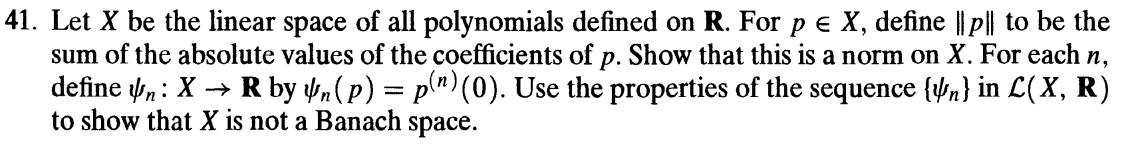
\includegraphics[width=1\textwidth]{13-41.png}
\end{figure}
\end{question}
\begin{solution} We first show that $\lVert \> \rVert:X \to \mathbb{R}$
given is a norm on $X$. First of all, 
\ 
\end{solution}

\newpage

\begin{question}[2. Royden 14-18]
\hfill
\begin{figure}[h!]
  \centering
    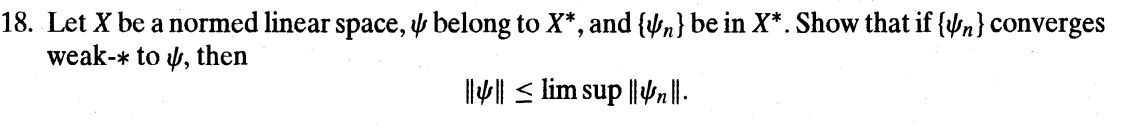
\includegraphics[width=1\textwidth]{14-18.png}
\end{figure}
\end{question}
\begin{solution}
As $\{ \psi_n \}$ is weak-* convergent to $\psi$, we have 
\eQb
\psi_n(x) &\to& \psi(x),
\eQe
for all $x \in X$. Let $x \in X$.
As $| \cdot |$ is continuous on $\mathbb{R}$,
it follows that
\eQb
\lim_{n \to \infty} |\psi_n(x)| &=& |\psi(x)|. 
\eQe 
As $|\psi_n(x) | \leq ||\psi_n || \cdot ||x||$, 
\eQb
|\psi(x)| &=& \lim_{n \to \infty} |\psi_n(x)| \\
&=& \limsup_{n \to \infty} |\psi_n(x)| \\ 
&\leq&\limsup_{n \to \infty} ||\psi_n || \cdot ||x|| \\
&=& ||x|| \limsup_{n \to \infty} ||\psi_n||.
\eQe
Since $x \in X$ was arbitrary,  it follows that
\eQb
||\psi|| &\leq& \limsup_{n \to \infty} ||\psi_n||, 
\eQe
as desired. \hfill $\qed$
\end{solution}

\newpage

\begin{question}[3. Royden 14-23]
\hfill
\begin{figure}[h!]
  \centering
    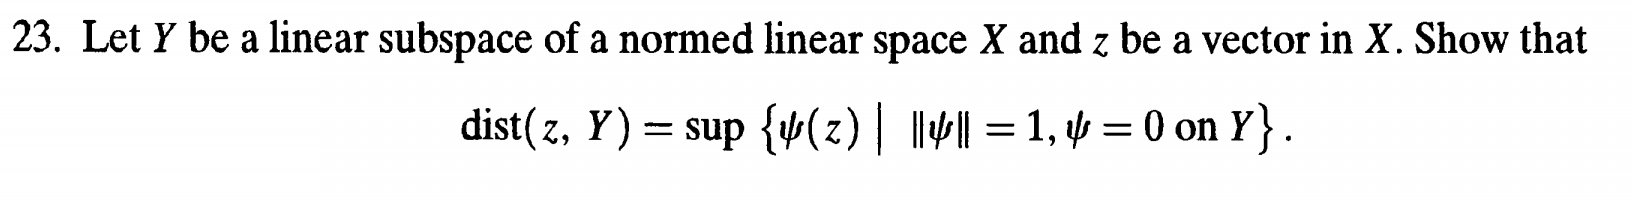
\includegraphics[width=1\textwidth]{14-23.png}
\end{figure}
\end{question}
\begin{solution}
Consider a functional $p:X \to [0,\infty)$ be defined by
\eQb
p = \begin{cases}
    0, & \text{if $x \in Y$} \\
    ||x||, & \text{otherwise}.
  \end{cases}
\eQe
We first show that $p$ is positively homogeneous. Let $\lambda > 0$. 
Let $x \in Y$, then as $Y$ is a linear subspace of $X$, $\lambda x \in Y$.
It follows that
\eQb
p(\lambda x) &=& 0 \\
&=& \lambda p(x). \\
\eQe 
Let $x \notin Y$. It follows that $\lambda x \notin Y$, as otherwise
we get a contradiction that $x \in Y$ from the linear subspace property
of $Y$. It follows that 
\eQb
p(\lambda x) &=& ||\lambda x || \\
&=& |\lambda | ||x|| \\
&=& \lambda ||x|| \\
&=& \lambda p(x).
\eQe
Hence, we have shown that $p$ is positively homogeneous. Now, we show that
$p$ is sub-additive. 
Let $x,y \in Y$. Then, it follows that
\eQb
p(x+y) &=& 0 \\
&=& p(x) + p(y). \\
\eQe  
Hence, $p(x+y) \leq p(x) + p(y)$ holds. Let $x,y \notin Y$. Then, 
by the triangle inequality of norm, it
follows that
\eQb
p(x+y) &=& || x + y|| \\
&\leq& ||x| + ||y|| \\
&=& p(x) + p(y). \\
\eQe
Let $x \in Y$ and $y \notin Y$. It follows that
\eQb
p(x+y) &=& || x + y || \\
&\leq& ||x|| + ||y|| \\
&=& 0 
\eQe  
\end{solution}

\newpage

\begin{question}[4. Royden 15-12]
\hfill
\begin{figure}[h!]
  \centering
    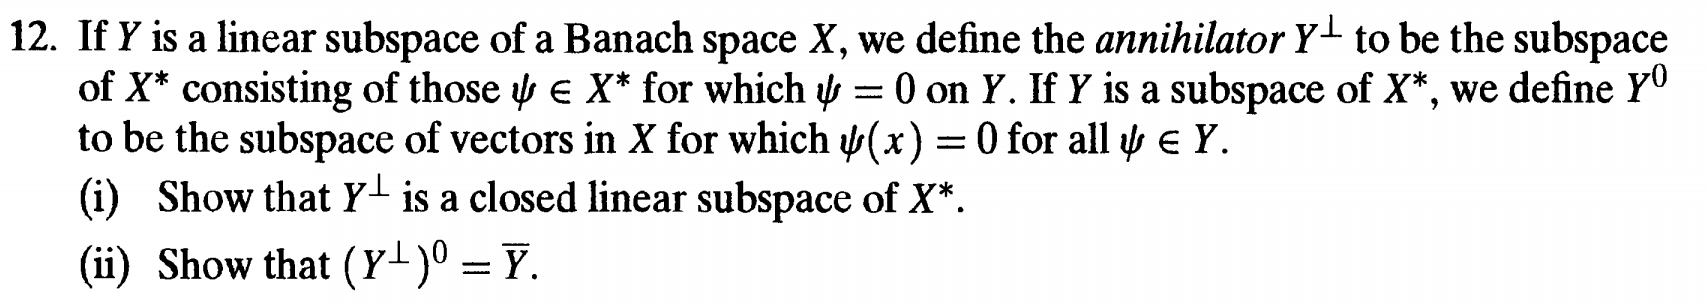
\includegraphics[width=1\textwidth]{15-12.png}
\end{figure}
\end{question}
\begin{solution}
\textit{Let $\mathcal{A}$ be an algebra of continuous real-valued functions on a compact Hausdorf space $X$ that separates points. Show that either $\bar {\mathcal{A}}=C(X)$ or there is a point $x_0 \in X$ for which $\bar{\mathcal{A}}=\{f \in C(X)|f(x_0)=0\}$}.  \\ 

To solve this problem, it suffices to prove that $\bar{A}=C(X)$ assuming $\bar{\mathcal{A}}\neq \{f \in C(X)|f(x_0)=0\}$, i.e.,  $\forall x \in X, \exists f_x\in C(X)$, s.t.  $f_x(x) =y_x\neq 0$. Then, the open interval $I_x=(y_x-\delta, y_x+ \delta)$ where $0<\delta<|y_x|$, is mapped to an open interval $O_x=f_x^{-1}(I_x) \subset X$ where $x \in O_x$.   Therefore, $X\subseteq \cup_{x \in X}O_x$. Since the foregoing is an open cover of a compact space $X$,  it contains a finite subcover      $\cup_{i=1}^nO_{x_i}$.  By construction, $0 \notin f_{x_i}(O_{x_i})$. Thus $g=\sum_{i=1}^n f^2_{x_i}$ is in $A$ and takes strictly positive values on $X$.  \\ 

Define $h:K\cup\{0\}\rightarrow R_+$ as follows\\
$$h(x)=\begin{cases}
1/x & \text{ if } x \in K\\
0 & \text{ if } x =0\\
\end{cases}$$\\  

By Proposition 20, since $X$ is compact and $g$ is a continuous mapping, the range of $g$, $K=g(X)$, is compact, which in the case of a real-valued range means that it is closed and bounded. Furthermore, since $K$ is closed and $0\notin K$, it is not possible to have a  sequence in $K$ converging to $0$. Therefore, $0 \notin \bar{K}=K$, which implies that  $h(x)$ is continuous on $D=K\cup\{0\}$\\

Now, since $h\in C(K)$, by Stone-Weierstrass, given  $\epsilon >0$, there exists $p_{n}$, a polynomial, s.t.\\

$$|h(x)-p_{n}(x)|<\epsilon /2 $$\\

for all $x \in K$. Since the above implies that $|p_n(0)|< \epsilon/2$  \\
 
$$|h(x)-(p_{n}(x)-p_n(0))|\leq |h(x)-p_{n}(x)|+|p_n(0))|<\epsilon $$\\

where $p^*_n(x)=p_{n}(x)-p_n(0)$ (and thus $p^*_n(0)=0$, which trivially guarantees the uniform convergence on $K\cup\{0\}$). Therefore, $p^*_n$ is continuos on $D$, and $p^*_n \circ g \in A$. Since $p^*_n$ converges uniformly to $h$ and $g$ is continuous and bounded (and consequently uniformly continuous on a compact set, $p^*_n\circ g \rightarrow 1/g$ uniformly. Therefore, $1/g \in \bar {A}$, which together with the fact that $g \in A$, implies that $1 \in \bar {A}$. This generates the family of constant functions in $A$.  By the Stone-Weierstrass Approximation, $\bar {A}$ is dense in $C(X)$. Since $\bar{A}$ is closed, this implies that $\bar {A}=C(X)$. \\
\end{solution}
\end{document}
